Exercise 1.2 gives the age $x_{1}$, measured in years, as well as the selling price $x_{2}$, measured
in thousands of dollars, for $n = 10$ used cars. These data are reproduced as follows:
\begin{center}
    \small
    \begin{tabular}{c|cccccccccc} % chktex 44
        $x_{1}$ & 1 & 2 & 3 & 3 & 4 & 5 & 6 & 8 & 9 & 11 \\
        \hline % chktex 44
        $x_{2}$ & 18.95 & 19.00 & 17.95 & 15.54 & 14.00 & 12.95 & 8.94 & 7.49 & 6.00 & 3.99
    \end{tabular}
\end{center}
\begin{enumerate}[label= (\alph*)]
    \item Use the results of Exercise 1.2 to calculate the squared statistical distances ${\left(\textbf{x}_{j} - \bar{\textbf{x}}\right)}^{\prime}\textbf{S}^{-1}\left(\textbf{x}_{j} - \bar{\textbf{x}}\right)$, $j=1,2,\dots,10$, where $\textbf{x}_{j}^{\prime} = [x_{j1}, x_{j2}]$.
    \[
        \bar{\textbf{x}}
        =
        \begin{bNiceArray}{c}
            5.2 \\
            12.4810
        \end{bNiceArray}
        \hspace{0.2cm}
        \textbf{S}
        =
        \begin{bNiceArray}{cc}
            10.6222 & -17.7102 \\
            -17.71102 & 30.8544
        \end{bNiceArray}
        \Rightarrow
        \textbf{S}^{-1}
        =
        \begin{bNiceArray}{cc}
            2.1898 & 1.2569 \\
            1.2569 & 0.7539
        \end{bNiceArray}
    \]
    \[
        \textbf{d}^{2}
        =
        {(\textbf{x}_{j} - \bar{\textbf{x}})}^{\prime}
        \textbf{S}^{-1}
        (\textbf{x}_{j} - \bar{\textbf{x}})
        =
    \]
    \[
        =
        {
        \begin{bNiceArray}{c}
            x_{j1} - \phantom{0}5.2000 \\
            x_{j2} - 12.4810
        \end{bNiceArray}
        }^{\prime}
        \begin{bNiceArray}{cc}
            2.1898 & 1.2569 \\
            1.2569 & 0.7539
        \end{bNiceArray}
        \begin{bNiceArray}{c}
            x_{j1} - \phantom{0}5.2000 \\
            x_{j2} - 12.4810
        \end{bNiceArray}
    \]
    We could compute all $j = 1, 2, \dots, 10$ values of $\textbf{d}^{2}$ at once. Here, $\textbf{x}_{j}$ is $p \times 1 = 2 \times 1$ vector, putting them all into a matrix, $\textbf{X} = [\textbf{x}_{1}, \textbf{x}_{2}, \dots, \textbf{x}_{10}]$ is $p \times n = 2 \times 10$. If we compute 
    \[
        {
            \left(
                \underset{(2 \times 10)}{\textbf{X}}
                -
                \underset{(2 \times 1)}{\bar{\textbf{x}}}
                \underset{(1 \times 10)}{\textbf{1}}
            \right)
        }^{\prime}
        \underset{(2 \times 2)}{\textbf{S}^{-1}}
        \left(
            \underset{(2 \times 10)}{\textbf{X}}
            -
            \underset{(2 \times 1)}{\bar{\textbf{x}}}
            \underset{(1 \times 10)}{\textbf{1}}
        \right)
    \]
    directly, the output is a $10 \times 10$ matrix where the squared distances are on the diagonal. We can save ourselves from the unnecessary multiplication of the off-diagonal elements by using element-wise multiplication with $\odot$:
    \[
        \textbf{d}^{2}
        =
        {\left(\textbf{x}_{j} - \bar{\textbf{x}}\right)}^{\prime}
        \textbf{S}^{-1}
        \left(\textbf{x}_{j} - \bar{\textbf{x}}\right)
        =
    \]
    \[
        =
        \text{diag}
        \left\{
            {\left(\textbf{X} - \bar{\textbf{x}}\textbf{1}\right)}^{\prime}
            \textbf{S}^{-1}
            \left(\textbf{X} - \bar{\textbf{x}}\textbf{1}\right)
        \right\}
        =
        ({\left(\textbf{X} - \bar{\textbf{x}}\textbf{1}\right)}^{\prime}
        \textbf{S}^{-1})
        \odot
        {\left(\textbf{X} - \bar{\textbf{x}}\textbf{1}\right)}^{\prime}
        =
    \]
    \[
        =\left(
            \begin{bNiceArray}{rr}
                -4.2 &  6.4690 \\
                -3.2 &  6.5190 \\
                -2.2 &  5.4690 \\
                -2.2 &  3.0590 \\
                -1.2 &  1.5190 \\
                -0.2 &  0.4690 \\
                0.8 & -3.5410 \\
                2.8 & -4.9910 \\
                3.8 & -6.4810 \\
                5.8 & -8.4910
            \end{bNiceArray}
            \begin{bNiceArray}{cc}
                2.1898 & 1.2569 \\
                1.2569 & 0.7539
            \end{bNiceArray}
        \right)
        \odot
        \begin{bNiceArray}{rr}
            -4.2 &  6.4690 \\
            -3.2 &  6.5190 \\
            -2.2 &  5.4690 \\
            -2.2 &  3.0590 \\
            -1.2 &  1.5190 \\
            -0.2 &  0.4690 \\
             0.8 & -3.5410 \\
             2.8 & -4.9910 \\
             3.8 & -6.4810 \\
             5.8 & -8.4910
        \end{bNiceArray}
        =
    \]
    \[
        =
        \begin{bNiceArray}{rr}
            -1.0661 & -0.4023 \\
             1.1866 &  0.8924 \\
             2.0566 &  1.3577 \\
            -0.9726 & -0.4591 \\
            -0.7185 & -0.3632 \\
             0.1515 &  0.1022 \\
            -2.6990 & -1.6640 \\
            -0.1419 & -0.2432 \\
             0.1751 & -0.1096 \\
             2.0282 &  0.8890
        \end{bNiceArray}
        \odot
        \begin{bNiceArray}{rr}
            -4.2 &  6.4690 \\
            -3.2 &  6.5190 \\
            -2.2 &  5.4690 \\
            -2.2 &  3.0590 \\
            -1.2 &  1.5190 \\
            -0.2 &  0.4690 \\
             0.8 & -3.5410 \\
             2.8 & -4.9910 \\
             3.8 & -6.4810 \\
             5.8 & -8.4910
        \end{bNiceArray}
        =
        \begin{bNiceArray}{c}
            1.8753 \\
            2.0203 \\
            2.9009 \\
            0.7353 \\
            0.3105 \\
            0.0176 \\
            3.7329 \\
            0.8165 \\
            1.3753 \\
            4.2153
        \end{bNiceArray}
    \]
    \item Using the distances in Part a, determine the proportion of the observations falling
    within the estimated 50\% probability contour of a bivariate normal distribution.
    \vspace{0.2cm}
    \par
    The Chi-square value where 50\% of the data is inside is found using the inverse CDF of a Chi-squared with $p = 2$ degrees of freedom, $F^{-1}(\text{prob} = 0.50| p = 2) = 1.3863$. Using the output from (a), there are 5 values less than 1.3863. Out of 10 total observations that makes 0.50 of the data. This is exactly what we'd expect under normality.

    \item Order the distances in Part a and construct a chi-square plot.
    
    \begin{figure}[H]
        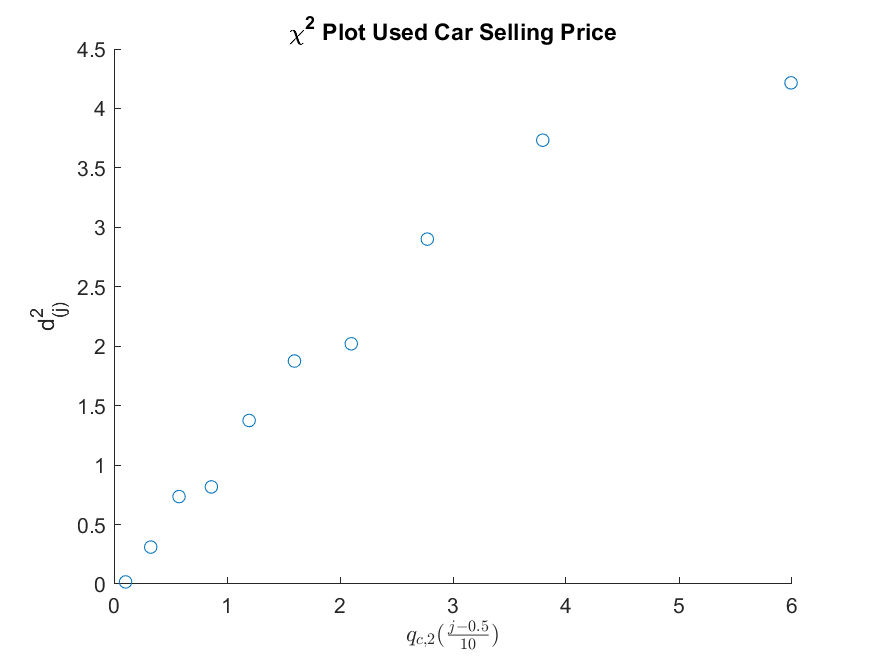
\includegraphics[scale=0.8]{./matlab/chapter-4/sol4.26c.png}
    \end{figure}

    \begin{center}
        \begin{tabular}{ccc}
            \hline % chktex 44
            $j$ & $d_{(j)}^{2}$ & $q_{c, 2}\left(\frac{j-\frac{1}{2}}{10}\right)$ \\
            \hline % chktex 44
            1  & 0.0176 & 0.1026 \\
            2  & 0.3105 & 0.3250 \\
            3  & 0.7353 & 0.5754 \\
            4  & 0.8165 & 0.8616 \\
            5  & 1.3753 & 1.1957 \\
            6  & 1.8753 & 1.5970 \\
            7  & 2.0203 & 2.0996 \\
            8  & 2.9009 & 2.7726 \\
            9  & 3.7329 & 3.7942 \\
            10 & 4.2153 & 5.9915 \\
            \hline % chktex 44
        \end{tabular}
    \end{center}
    \item Given the results in Parts b and c, are these data approximately bivariate normal?
    Explain.
    \vspace{0.2cm}
    \par
    In part (b) we found that 50\% of our data is within the contour of what we would expect if the data was normally distributed. In part (c), the $\chi^{2}$-plot shows our data to be roughly linear. For these reasons we could conclude that there is evidence that used car sale data is normally distributed.
\end{enumerate}